\documentclass[12pt]{article}

\usepackage{graphicx}
\usepackage{svg}

\newcommand{\code}[1]{\texttt{#1}}

\usepackage[utf8]{inputenc}
\usepackage[
    twoside,
    top=1in,
    bottom=0.75in,
    inner=0.5in,
    outer=0.5in
]{geometry}

\usepackage{tcolorbox}
\tcbuselibrary{skins}
\usepackage{minted}
\usepackage{color}
\usepackage{tikz}
\usetikzlibrary{calc}
\usepackage{tabularx,colortbl}
\usepackage{amsfonts,amsmath,amssymb}
\usepackage{titling}
\usepackage{mathrsfs}
\usepackage{calc}
\usepackage{graphicx}
\usepackage{svg}
\usepackage[
    backend=biber,
    style=authoryear,
    sorting=nyt
]{biblatex}

\addbibresource{bibliography.bib}


\title{Homework Template and Samples}
\author{Heather Tweedie}
\date{March 2023}

\linespread{1.25}

\begin{document}

%%%% Format Running Header %%%%%
\markboth{\theauthor}{\thetitle}

%%%% Insert the Title Information %%%
\maketitle


%%%% General Description of the Document %%%%
\begin{abstract}

\end{abstract}

\section{Introduction}
\section{Data used}

The data used in this study were obtained from the Global Historical Climate Network (GHCN). GHCN-Daily (GHCND) (Menne et al., 2012a) 
is a database of daily weather summaries featuring data from over 80,000 stations in 180 countries (Menne et al., 2012). Approximately 
two thirds of the stations report precipitation data only, however many stations report maximum and minimum temperatures, snowfall and 
depth in addition. The data come from a number of global sources including the National Oceanic and Atmospheric Administration, the 
European Climate Assessment and Dataset, and the South African Weather Service, and are subjected to automated, unsupervised quality 
assurance tests.

Only stations which are part of the GCOS Surface Network (GSN) were included in this study. As of March 2019, 1023 stations were part 
of this network (Oakley, 2018), providing an approximately uniform coverage of the globe with high-quality data of a good length 
(GCOS, n.d.) (Figure 1).

    \begin{figure}
        \centering
        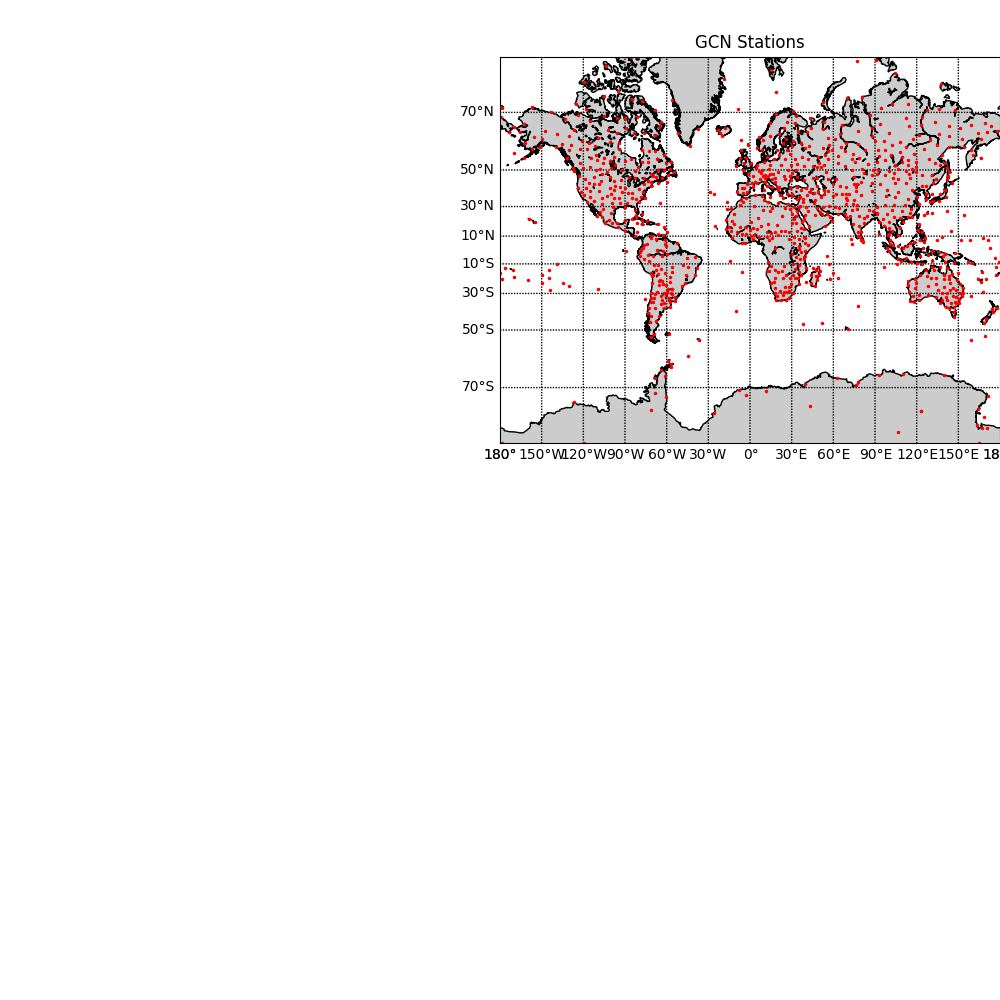
\includegraphics[scale = 1.2]{all_stations.png}
        \caption{All stations included in the GCOS Surface Network (GSN). Stations are marked as red points and plotted on a basemap
         of the Mercator projection. The network provides a relatively uniform coverage of global land areas.}
        \label{fig:my_label}
    \end{figure}

\section{Predicting the weather}
\subsection{Methodology}


Initial processing of the data was carried out in the same way for both primary research questions. To further filter the stations used, 
the number of missing data points from the variable in question were counted; the stations with no or few gaps were focused upon for study. 
A station to investigate was selected on this basis, and the data for that station acquired from a course-provided directory of GSN station 
data files. Time-series data for the specified variable were then extracted from this file and stored in a separate \code{Variable} class 
with fields for the values and their corresponding dates.

\subsection{Results}
\section{Predicting the climate}
\subsection{Methodology}
\subsection{Results}
\end{document}
